\documentclass{article}
\usepackage[T1]{fontenc}
\usepackage[margin=22mm]{geometry}
\usepackage{tikz}
\title{Independent HyMeKo topological mapping}
\date{Created: 2026-10-10 01:43 +02:00}
\begin{document}\maketitle
\noindent Status: proposed protected-kernel extension; implementation not started.
ETA after kernel approval: 60--90 minutes for the bounded batch operation,
analytical checks and IR integration. Full paper reproduction is a later,
separately specified scope. No speedup is currently measured.
\section*{Requested boundary}
The user explicitly requires independence from Nagare and Transformation.
Neither repository is edited, imported or built. Use existing Core compilation
and canonical IR; Graph owns graph operations, SBSH the spatial partition.
No parser, canonical model, training framework, graph traversal or example
pipeline is duplicated. No new dependency, repository, worktree or backend.
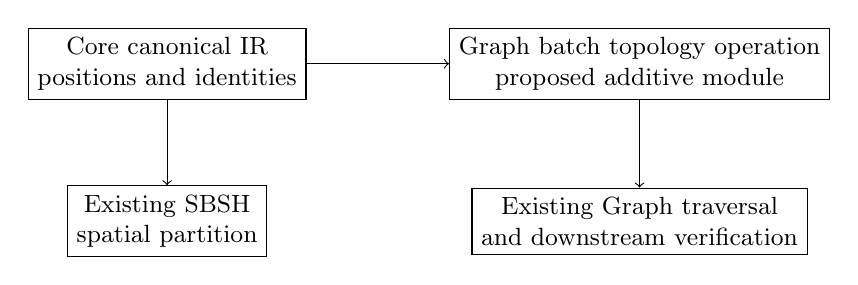
\begin{tikzpicture}[every node/.style={draw,align=center,font=\small}]
\node (ir) at (0,0) {Core canonical IR\\positions and identities};
\node (g) at (6,0) {Graph batch topology operation\\proposed additive module};
\node (s) at (0,-2) {Existing SBSH\\spatial partition};
\node (v) at (6,-2) {Existing Graph traversal\\and downstream verification};
\draw[->] (ir)--(g);\draw[->] (ir)--(s);\draw[->] (g)--(v);
\end{tikzpicture}

\section*{Discovery and source}
The current Graph workspace already compiles Core and Tensor without either
excluded repository. PositionProvider, IrPositions, SbshScene, SignedGraph and
direct-IR graph searches exist. GNG was not found in the inspected Graph/Tensor
source or symbols. SBSH's orthtree partitions given points; it does not learn a
prototype graph. The numerical method is from Siow et al., Biomimetics 2024,
9(9):560, DOI 10.3390/biomimetics9090560. Source code was not found in the
paper-linked repository's main tree; this will be an explicitly specified
implementation, not bitwise compatibility with unavailable author code.
\section*{Concrete first implementation}
Propose a generic batch point-to-graph operation in the canonical graph owner,
not a domain-specific robot trainer. The first independently verifiable unit
is equations 16--28 and 30--35: nearest two prototypes, separately normalized
winner and neighbor updates using the pre-batch graph, replacement of edges by
winner-pair links, isolated-node removal, error discount, and error-driven
midpoint growth. Inputs are positions and a caller-declared initial graph;
output is a learned graph and a deterministic step receipt. It does not promise
collision-free navigation. Inactive-node random deletion and multi-scale
initialization/scheduling are excluded from the first bounded contract.
\begin{verbatim}
BatchGasConfig { winner_rate, neighbour_rate, epsilon,
                 error_discount, growth_discount, growth_quantile,
                 max_nodes, max_distance_evaluations }
BatchGas::new(positions, graph, config) -> Result<BatchGas, GasError>
BatchGas::step(points) -> Result<StepReceipt, GasError>
BatchGas::positions() -> &[[f64; 3]]
BatchGas::graph() -> &SignedGraph
StepReceipt { evaluated_pairs, nodes_before, nodes_after,
              edges_after, removed, inserted }
\end{verbatim}
The configuration will have finite bounds and stable tie handling. The existing
SignedGraph owns connectivity; no second canonical hypergraph is introduced.
The floating point buffers are algorithm state. A later IR binding consumes
canonical identities via PositionProvider and retains explicit input/output
provenance; do not invent a source parser or recompile every iteration.
\section*{Files and protected scope}
Unprotected preparation in this turn:
\begin{verbatim}
docs/plans/2026-10-10-independent-topology-map/plan.tex
docs/plans/2026-10-10-independent-topology-map/plan.pdf
docs/plans/2026-10-10-independent-topology-map/plan.tikz
docs/plans/2026-10-10-independent-topology-map/plan.mmd
reports/2026-10-10-independent-topology-map.md and evidence directory
\end{verbatim}
Protected implementation proposal, not applied:
\begin{verbatim}
hymeko_graph/src/lib.rs                 (one additive public module)
hymeko_graph/src/neural_gas/mod.rs      (state and public contract)
hymeko_graph/src/neural_gas/batch.rs    (one batch implementation)
hymeko_graph/tests/neural_gas.rs        (analytical verification)
SYMBOLS.md                             (provider-generated)
\end{verbatim}
CORE.YAML item affected by the proposal: hymeko\_graph. Its explicit gate
requires approval after this written justification and migration plan.
Current edits affect no protected item. Tensor and SBSH need no kernel changes.
Public changes are additive; old consumers keep their current pins and behavior.
Rollback removes only newly added module/test files and its one export.
No commit or push is requested for this Graph work.
\section*{Verification and resource contract}
First establish the existing independent foundation with the selected
ir\_direct and scene\_ir correctness targets. Inspect the resolved dependency
closure and require zero Nagare, Formats, Query, Emitter and Geometry crates.
After approval, test hand-calculated winner/neighbor deltas, synchronous updates,
Euclidean (not squared) accumulated error, graph replacement, remapping after
deletion, percentile interpolation, capped midpoint insertion, tie ordering,
empty/NaN/Inf rejection and failure atomicity. Compare graph reachability through
existing Graph traversal; never copy BFS into the learner or tests.
Fix maximum 4096 prototypes, 65536 points per call, coordinates bounded by
$10^6$, and an explicit distance-evaluation budget checked before mutation.
Use streaming pair-distance evaluation; do not allocate a full point-by-node
matrix. No allocation may follow unchecked input multiplication. Numerical
overflow must fail, never be treated as a large valid fitness.
No performance measurement in this preparation. Later benchmark opt-in only:
same input, precision, node budget, initialization and quality threshold;
include conversion and topology construction in end-to-end cost. Target 5x is
a hypothesis. Baseline implementations and hardware must be frozen first.
\section*{Paper ambiguities and risks}
Equations 14--15 index the final phase at a full-size batch but set its offset
to the same size, yielding an empty range. The prose instead avoids full-batch
learning. Section 3 states neighbor rate 0.01 while the experiment section uses
0.1. Neither ambiguity may be silently resolved and called an exact paper
reproduction. Freeze the bounded batch contract first; then document a schedule
interpretation and compare variants. Quantization error does not certify
connectivity, passage preservation, homotopy or collision freedom. Worst-case
quadratic point/prototype work needs explicit budget rejection, even if memory
is linear. Avoid nested thread pools and unexplained numerical reordering.
\section*{Execution addendum, 2026-10-10 01:59 +02:00}
The user explicitly approved this Graph extension at 01:46. The first bounded
batch operator is implemented under the proposed module and test paths. Added
read-only error observation and old-to-new / insertion-parent provenance in the
receipt support the planned numerical checks. Admission also caps initial edges
at 262144 and the configurable pair budget at 16777216. These additions tighten
the stated memory/work bounds; no dependency or existing algorithm changed.
The original pre-implementation proposal above is retained for provenance.
\end{document}
